\subsection{3D Druck}
\label{sec:3d_druck}

\ac{FDM} umgangssprachlich auch 3D Druck genannt ist eine Art der additiven Fertigung. Bei \ac{FDM} werden \ac{CAD} Modelle in viele einzelne Schichten aufgeteilt und diese dann Schicht für Schicht aufgebaut. Dabei wird ein Kunststoff in einem Druckkopf (Extruder) erwärmt und dann auf die vorherige Schicht aufgetragen. Dieser Vorgang wird solange wiederholt bis das \ac{CAD} Modell fertig gedruckt ist. \ac{FDM} ist eine der am meisten verbreiteten Methoden um 3D Objekte zu drucken. \ac{FDM} ist auch die Methode, die vom Projektteam gewählt wurde. Andere Formen des 3D"=Drucks wie \ac{SLA} oder \ac{SLS} funktionieren auf einem ähnlichen Prinzip, jedoch sind diese Methoden teurer, komplizierter und oft langsamer. Eine Darstellung des \ac{FDM} Verfahrens ist in Abbildung \ref{fig:fdm} zu sehen.

\begin{figure}[H]
    \centering
    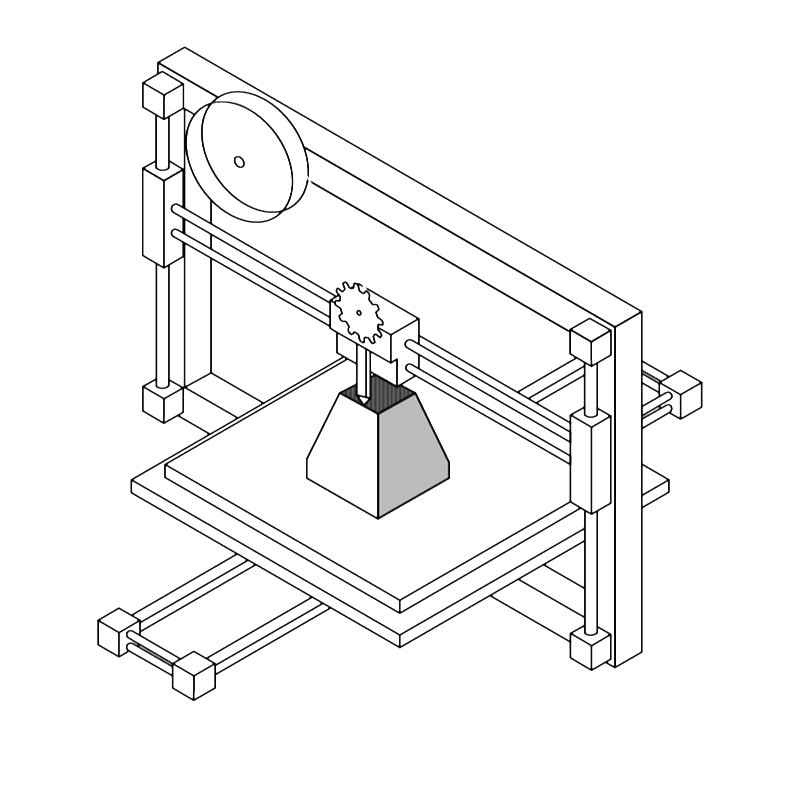
\includegraphics[width=0.5\textwidth]{images/fdm.png}
    \caption{Schematische Darstellung des \ac{FDM} Verfahrens \citev{3d_druck}}
    \label{fig:fdm}
\end{figure}

\subsubsection{\ac{SLA}}

\ac{SLA} ist ein Verfahren bei dem ein flüssiges Harz mit einem UV-Laser selektiv, Schicht für Schicht, ausgehärtet wird. Dieser Vorgang wird solange wiederholt bis das \ac{CAD} Modell fertig gedruckt ist. \ac{SLA} ist eine der teuersten Methoden um 3D Objekte zu drucken \citev{stereolithografie}. Eine Darstellung des \ac{SLA} Verfahrens ist in Abbildung \ref{fig:sla} zu sehen.

\begin{figure}[H]
    \centering
    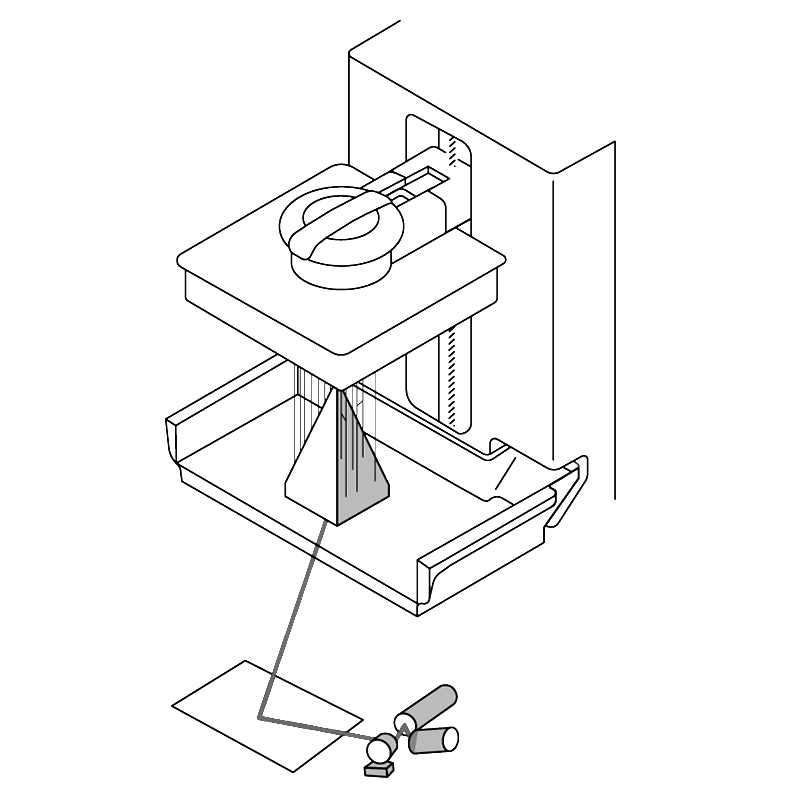
\includegraphics[width=0.5\textwidth]{images/sla.png}
    \caption{Schematische Darstellung des \ac{SLA} Verfahrens \citev{3d_druck}}
    \label{fig:sla}
\end{figure}

\subsubsection{\ac{SLS}}

Bei \ac{SLS} wird Kunststoffpulver von einem Laser geschmolzen. Sobald eine Ebene vollendet ist wird neues Pulver aufgetragen und der Vorgang wird wiederholt \citev{selektives_laser_sintern}. \ac{SLS} hat unter anderem den Vorteil, dass Bauteile keine Stüztstrukturen benötigen. Eine Darstellung des \ac{SLS} Verfahrens ist in Abbildung \ref{fig:sls} zu sehen.

\begin{figure}[H]
    \centering
    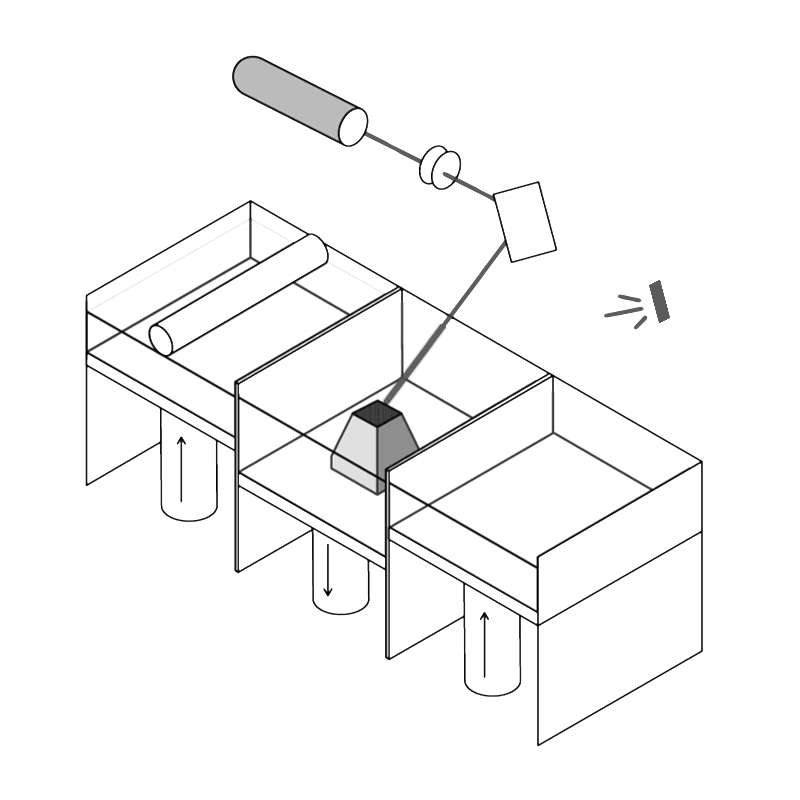
\includegraphics[width=0.5\textwidth]{images/sls.png}
    \caption{Schematische Darstellung des \ac{SLS} Verfahrens \citev{3d_druck}}
    \label{fig:sls}
\end{figure}